\chapter{Introduction 简介}
\begin{figure}[ht]
  \centering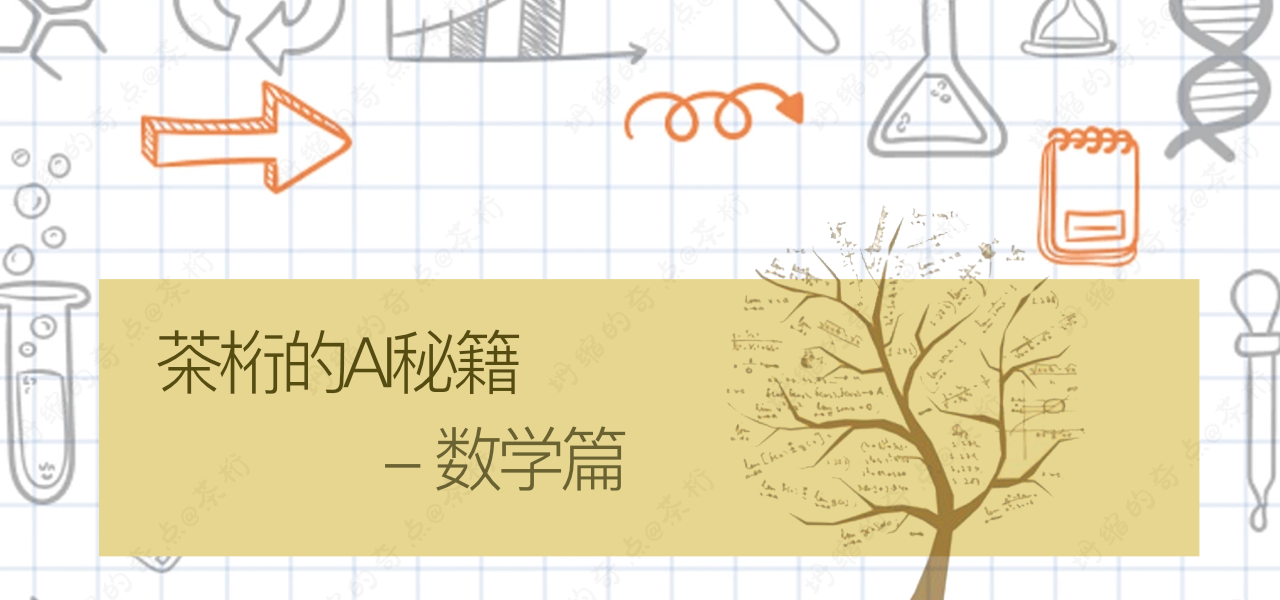
\includegraphics[width=1\linewidth]{asset/茶桁的AI秘籍_数学篇.png}
\end{figure}

\newpage
\section{导言}

Hi, 大家好。我是茶桁。

在\href{https://mp.weixin.qq.com/mp/appmsgalbum?__biz=MzA4NzE4MDQzMg==&action=getalbum&album_id=3035995870421073928&scene=173&subscene=&sessionid=undefined&enterid=0&from_msgid=2648748542&from_itemidx=1&count=3&nolastread=1#wechat_redirect}{Python篇} \href{https://mp.weixin.qq.com/s/mbnag65xDP-1Ct_81Byn5g}{PDF发布}后, 我又制作了\href{https://mp.weixin.qq.com/mp/appmsgalbum?__biz=MzA4NzE4MDQzMg==&action=getalbum&album_id=3074770001140400130&from_itemidx=1&from_msgid=2648748768#wechat_redirect}{数学篇}。
  
在整个连载的过程中, 后台有小伙伴留言说想要电子书, 在公众号内进行阅读还是有些不太方便。在平时, 茶桁其实很多的知识和内容都是来自于公众号, 当然, 更多的是来自于书本。

咱们整个数学篇基本上都属于基础理论知识, 概念、公式、推导比较多, 但是为了让大家将数学概念和程序关联上, 在其中也涉及到了一些编码的部分, 也讲解了人工智能上数学是怎么应用的, 比如在Chapter6中, 我就给大家讲解了\hypertarget{数学如何运用于AI}{数学如何运用于AI}.

所有在数学篇内涉及到的程序代码, 也都在代码仓库中可以找到: 可以选择一个自己访问顺畅的进行拉取。

\begin{itemize}
  \item \href{https://github.com/hivandu/AI_Cheats}{Github}
  \item \href{https://gitee.com/hivandu/ai_cheats}{Gitee}
\end{itemize}

这个仓库内包含了目前为止整个《AI秘籍》的全部代码以及数据集, 方便小伙伴下来之后进行练习。那仓库中的代码截至运行时间是2023年12月26日, 为什么要写这个, 因为有些包里的一些参数会做一些变动, 到目前为止这些代码都可正常运行, 假如过若干时间之后大家发现代码运行不了, 可以去看看包的官方文档, 也可以后台留言给我进行说明, 我会对电子书进行更新。

由于「数学篇」是一个付费专辑, 所以这本电子书并不是免费发放的, 仅针对已经付费的用户发送, 其余小伙伴想要阅读, 只能是进行购买了。不过本电子书是长期修正更新的, 在购买之后, 如果电子书内容进行了刊正, 则会对其进行更新, 并再次发送给已经购买的用户。还望小伙伴们在观看的过程中能够指出我的错误, 以便我对本电子书进行维护。

和制作Python篇的电子书的时候不同, 为了对数学篇进行付费的小伙伴们负责, 这次整个数学篇的电子书都一篇一篇进行了修正, 有些篇章更是重新写了一遍. 然后用Latex来重新设计和制作排版, 等于是整本书基本上都重构了一遍.

在修正的过程中才发现, 之前很多地方都有错误,有些错误甚至都是有误导性的. 在此要跟已经购买过数学篇的小伙伴们说声抱歉. 

当然, 虽然已经尽力的去寻找并且修正, 但也许不可避免的仍然还会有些错漏的地方, 在整个重新制作的过程中, 主要将经历放在了公式和概念上, 首先是争取对同学们不造成误导, 其次是有些地方的推导重新推导了, 争取能更容易进行理解. 在阅读过程中, 如果有小伙伴发现了错误或者遗漏, 还望给我留言, 我会尽快修正.

本电子书加入了版本号, 在每一章节的右下角部分, 如果有更新, 版本号都会有所变化. 并且在首页二维码下方的日期也会变化.

本电子书在\href{https://github.com/hivandu/Ebook_AI_Math}{Github上公开了源码}, 不过由于内容还是付费内容, 所其中章节并未上传, 仅上传了主文件和一些设置内容. 不过对于想研究电子书制作的的小伙伴已经足够了.

最后, 感谢大家的支持, 特别感谢付费支持的小伙伴们。还望关注「坍缩的奇点」, 日后咱们会有一些干货分享给大家, 也会和大家一起来完成一些企业项目, 帮助小伙伴们更快的步入到实际工作中去。

\begin{figure}[ht]
  \centering
  
\includegraphics[width=0.6\linewidth]{asset/Capture-2023-11-02-164446.png}
  \caption{敬请关注「坍缩的奇点」,获取更多人工智能相关教程及资料。}
  \label{fig:img1_1}
\end{figure}